
\subsection{Controladores PID e Sistemas Dinâmicos de Primeira Ordem}

\hspace{4ex}O controlador PID, na realidade, pode ser visto como sendo uma família de controladores. As 3 ações de controle podem ser combinadas de diferentes maneiras, formando controladores que podem receber diferentes nomes, como: P, PI, PD, PID, conforme as ações de controle são, ou não, utilizadas.

\begin{enumerate}
    \item Controle Proporcional (P):
    \[u(t)=Kpe(t)\] 
    \[U(S)=KpE(S)\]
        \begin{itemize}
            \item O controlador proporcional é um amplificador, com ganho ajustável (K);
            \item O aumento do ganho K, diminui o erro de regime;
            \item Em geral, o aumento de K torna o sistema mais oscilatório, podendo instabilizá-lo;
            \item Melhora o regime e piora o transitório, sendo bastante limitado.
        \end{itemize}
        
    \item Controle Proporcional + Integral (PI):
    \[u(t)=Kp(e(t)+\frac{1}{\tau i}\int_{0}^{t}e(\tau)d\tau)\]
    \[U(S)=\frac{(KpS+Ki)}{s}E(s)\]
        \begin{itemize}
            \item A ação integral do controlador move a variável de controle C(S) baseada na integral no tempo do erro, sendo: \[Ki=\frac{Kp}{\tau i}\], em que: \[\tau i\] é o tempo integrativo, ou tempo de \emph{reset}, com unidade da ordem de minutos;
            \item Zera o erro de regime, pois aumenta o tipo do sistema em 1 unidade;
            \item É utilizado quanto tempos resposta transitória aceitável e resposta em regime insatisfatória;
            \item Adiciona um pólo em p=0 e um zero em \[z=\frac{ki}{kp}=\frac{-1}{\tau i}\]
            \item Como aumenta a ordem do sistema, temos possibilidade de instabilidade diferente do sistema original. Pode degradar o desempenho do controlador em malha fechada.
        \end{itemize}
        
    \item Controle Proporcional + Derivativo (PD):
        \[u(t)=Kp(e(t)+\tau d\frac{de(t)}{dt})\]
        \[U(S)=(Kp+KdS)E(S)\]
        \begin{itemize}
            \item Sendo: \[Kd=Kp\tau d\] a constante derivativa, dada em minutos.
            \item Leva em conta a taxa de variaçao do erro;
            \item É utilizado quando temos resposta em regime aceitável e resposta transitória insatisfatória;
            \item Adiciona um zero em \[z=\frac{-Kp}{Kd}=\frac{-1}{\tau d}\]
            \item Introduz um efeito de antecipação no sistema, fazendo com que o mesmo reaja não somente à magnitude do sinal de erro, como também à sua tendência para o instante futuro, iniciando, assim, uma ação corretiva mais cedo;
            \item A ação derivativa tem a desvantagem de amplificar os sinais de ruído, o que pode causar um efeito de saturação nos atuadores do sistema.
        \end{itemize}
        
    \item Controle Proporcional + Integral + Derivativo (PID):
        \[u(t)=Kp(e(t)+\frac{1}{\tau i}\int_{0}^{t}e(\tau)d(\tau)+\tau d\frac{de(t)}{dt})\]
        \[U(S)=(Kp+\frac{Ki}{s}+KdS)E(S) => \frac{U(S)}{E(S)}=\frac{KdS^2+KpS+Ki}{S}\]
        \begin{itemize}
                    \item É utilizado quando temos resposta transitória e em regime insatisfatórias simultaneamente;
            \item Adiciona um pólo em p=0 e 2 zeros, que dependem dos parâmetros do controlador.
        \end{itemize}
        
    \item Implementação do Controlador PID:
        \begin{itemize}
            \item Diferentes equipamentos, de diferentes fabricantes, podem apresentar pequenas variações quanto à implementação do controlador PID. As duas implementações mais comumente utilizadas são: \textbf{Ideal} e \textbf{Paralelo}.
        \end{itemize}
        
    \item Modificações das Ações de Controle PID:
        \begin{itemize}
            \item Existem também diversas modificações, que poderão ser necessárias em cada implementação, dependendo de características do sistema que estiver sendo controlado, das condições de operações as quais o sistema será submetido e, até mesmo, do equipamento que será utilizado para implementação do controlador.
        \end{itemize}
        
        \begin{enumerate}
            \item Modificação na Ação Derivativa:
                \begin{itemize}
                    \item Filtro da Ação Derivativa
                        \begin{figure}[h]
                            \centering
                            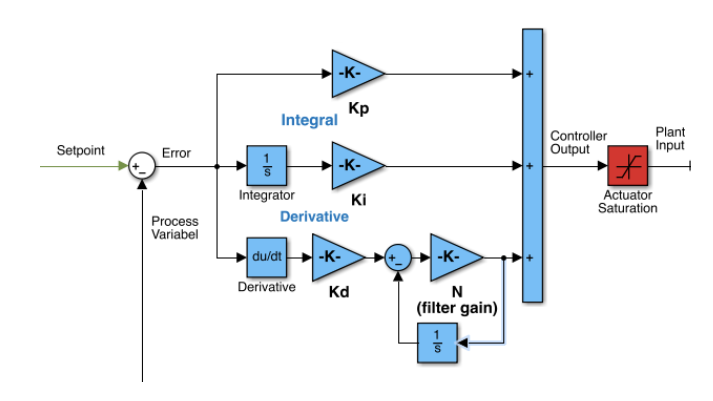
\includegraphics[width=15cm]{images/roteiro a/img ref teorico/filtro_de_acao_derivativa.png}
                            \caption{Filtro de Ação derivativa}
                            \label{fig:filtro_de_acao_derivativa}
                        \end{figure}
                    \item PI-D
                        \begin{figure}[h]
                            \centering
                            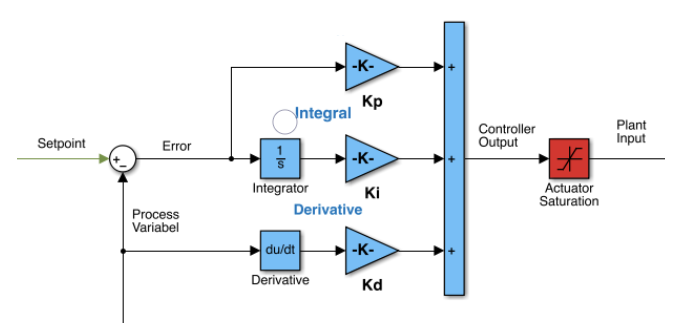
\includegraphics[width=15cm]{images/roteiro a/img ref teorico/pid.png}
                            \caption{PI-D}
                            \label{fig:pid}
                        \end{figure}
                        \begin{itemize}
                            \item Objetivo: Não derivar variações bruscas no sinal de referência. 
                        \end{itemize}
                        \newpage
                    \item I-PD
                         \begin{figure}[h]
                            \centering
                            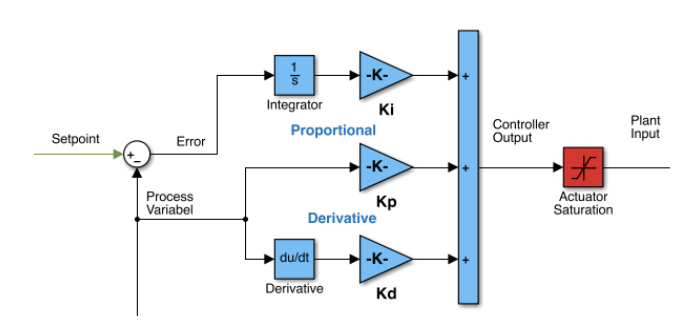
\includegraphics[width=15cm]{images/roteiro a/img ref teorico/ipd.png}
                            \caption{I-PD}
                            \label{fig:ipd}
                        \end{figure}
                        \begin{itemize}
                            \item Objetivo: Não derivar, nem amplificar variações bruscas no sinal de referência. 
                            \\
                        \end{itemize}
                \end{itemize} 
            \item Modificação na Ação Integrativa:
                \begin{itemize}
                    \item Filtro Anti-Windup (Anti-Reset Windup)
                \end{itemize}
                    \begin{figure}[h]
                            \centering
                            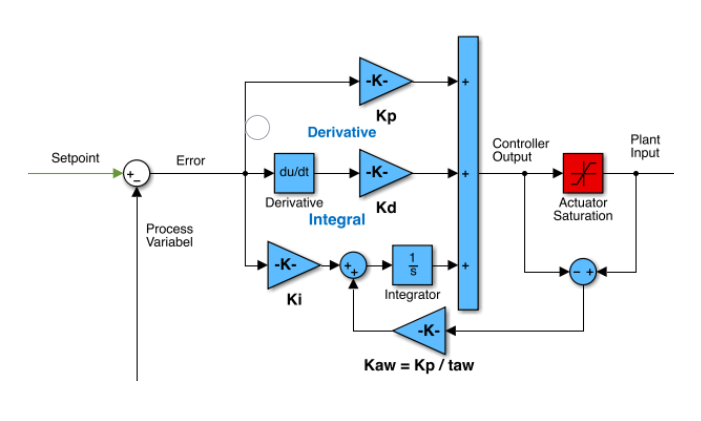
\includegraphics[width=15cm]{images/roteiro a/img ref teorico/filtro_anti_windup.png}
                            \caption{Filtro Anti-Windup (Anti-Reset Windup)}
                            \label{fig:filtro_anti_windup}
                        \end{figure}
        \end{enumerate}
\end{enumerate}
\newpage

\subsection{Sistemas de Segunda Ordem}
\hspace{4ex}Considere a seguinte equação diferencial de segunda ordem:
    \[a\frac{d^2e(t)}{dt^2}+b\frac{de(t)}{dt}+dc(t)=er(t)\]
Definindo:
    \[\frac{b}{a}=2\epsilon\omega_n; \hspace{4ex} \frac{d}{a}=\omega^2_n; \hspace{4ex} \frac{e}{a}=K;\]
onde \(\epsilon\) é o fator de amortecimento, \(\omega_n\) é a frequência natural e K é o ganho do sistema, temos:
    \[\frac{d^2c(t)}{dt^2}+2\epsilon\omega_n\frac{dc(t)}{dt}+\omega_n^2c(t)=Kr(t)\]
Aplicando Laplace com C.I. nulas: 
    \(\frac{C(s)}{R(s)}=\frac{K}{S^2+2\epsilon\omega_nS+\omega_n^2}\) 
    \newline
    \newline
Considerando K = \(\omega_n^2\): \(\frac{C(s)}{R(s)}=\frac{\omega_n^2}{S^2+2\epsilon\omega_nS+\omega_n^2}\)
    \newline
    \newline
Polos do sistema: \(S^2+2\epsilon\omega_n^2S+\omega_n^2=0\) => \(S=-\epsilon\omega_n\pm\omega_n\sqrt{\epsilon^2 -1}\)
    \newline
    \newline
Exemplos de sistemas de 2ª ordem: circuitos RLC, sistema massa-mola-atrito, servomecanismo de posição.
    \newline

Temos três casos:
\begin{enumerate}
    \item \(0 < \epsilon < 1\): Caso \textbf{SUBAMORTECIDO}. O sistema tem dois polos complexos conjugados e apresenta oscilações;
    \item \(\epsilon = 0\): Caso \textbf{CRITICAMENTE AMORTECIDO}. Dois polos reais e iguais. A partir deste valor de \(\epsilon\) o sistema passa a não ter mais oscilações;
    \item \(\epsilon > 1\): Caso \textbf{SOBREAMORTECIDO}. Dois polos reais e distintos. A medida que \(\epsilon\) aumenta, o comportamento do sistema se aproxima do comportamento de um sistema de 1ª ordem.
\end{enumerate}

\hspace{4ex} \underline{Resposta ao Degrau Unitário}

\begin{enumerate}
    \item Caso Subamortecido: 
        \[c(t)=1-\frac{e^{-\epsilon\omega_n t}}{\sqrt{1-\epsilon^2}}\sin(\omega_d t+\tan^{-1}\frac{\sqrt{1-\epsilon^2}}{\epsilon})\]
onde: \(\omega_d=\sqrt{1-\epsilon^2}\) é a frequência natural amortecida.
\newline
Se \(\epsilon=0\), então: \(c(t)=1-\cos\omega_n t\)

    \item Caso Criticamente Amortecido: \(c(t)=1-e^{-\omega_n t}(1+\omega_n t)\)

    \item Caso Sobreamortecido: 
    \[c(t)=1+\frac{\omega_n}{2\sqrt{\epsilon^2 -1}}(\frac{e^{-S_1 t}}{S1}-\frac{e^{-S_2 t}}{S2})\]
onde \(S_1=(\epsilon+\sqrt{\epsilon^2 -1})\omega_n\) e \(S_2=(\epsilon-\sqrt{\epsilon^2 -1})\omega_n\)
\newline
\end{enumerate}

\hspace{4ex} \underline{Especificações de Resposta Transitória}

\begin{figure}[h]
    \centering
    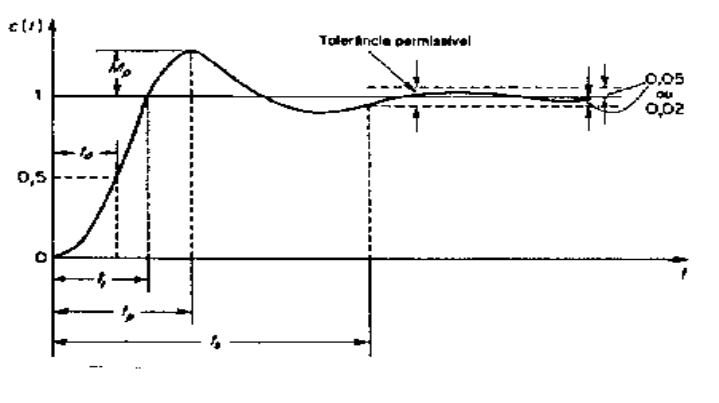
\includegraphics[width=15cm]{images/roteiro b/img ref teorico/curva.PNG}
    \caption{Curva com as Especificações da Resposta Transitória}
    \label{fig:curva}
\end{figure}

\hspace{4ex}Definições:

\begin{enumerate}
    \item \underline{Tempo de Subida}, \textbf{\(t_r\)}: É o tempo necessário para que a saída atinja pela primeira vez o seu valor final.
    \newline
    \[t_r=\frac{\pi-\beta}{\omega_n}; \hspace{4ex} onde \hspace{4ex} \beta=\tan^{-1}\frac{\sqrt{1-\epsilon^2}}{\epsilon}\]
    \newline
    \item \underline{Tempo de Pico}, \textbf{\(t_p\)}: É o instante de tempo em que a resposta atinge o primeiro pico de sobressinal.
    \[t_p=\frac{\pi}{\omega_d}\]
    \newline
    \item \underline{Máximo sobressinal (\textit{Overshoot})}, \textbf{\(M_p\)}: É o valor máximo de pico da curva de resposta medido a partir do valor final.
    \[M_p(\%)=\frac{c(t_p)-c(\infty))}{c(\infty)}x100\%\]
    \[c(t_p)=1+e^-({\frac{\epsilon\pi}{\sqrt{1-\epsilon^2}}})\]
    Logo: \newline
    \[M_p(\%)=100e^-({\frac{\epsilon\pi}{\sqrt{1-\epsilon^2}}})\]
    OBS: O sobressinal máximo depende do valor do coeficiente de amortecimento \(\epsilon\).
    \newline
    \item \underline{Tempo de Acomodação (Estabilização), \(t_s\)}: É o tempo necessário para que a resposta alcance e permaneça dentro de uma faixa em torno do valor final. Esta faixa é especificada por uma porcentagem absoluta do valor final (2\% ou 5\%).
    
    \[t_s=\frac{4}{\epsilon\omega_n} \hspace{8ex} (criterio \hspace{1ex} de \hspace{1ex} 2\%)\]
    
    \[t_s=\frac{3}{\epsilon\omega_n} \hspace{8ex} (criterio \hspace{1ex} de \hspace{1ex} 5\%)\]
    
OBS: As curvas e especificações calculadas são válidas somente para sistemas de 2ª ordem ideal, cuja função de transferência apresenta dois polos e nenhum zero.
    \[\frac{C(S)}{R(S)}=\frac{\omega_n^2}{S^2+2\epsilon\omega_nS+\omega_n^2)}\]
\end{enumerate}

\subsection{Sistemas de Segurança Instrumentados ou Intertravamentos}\hspace{4ex}

\subsection{Sistemas Dinâmicos na Configuração de Controle em Cascata}\hspace{4ex}